\begin{figure}[H]
\centering
%
\begin{subfigure}{0.95\textwidth}
  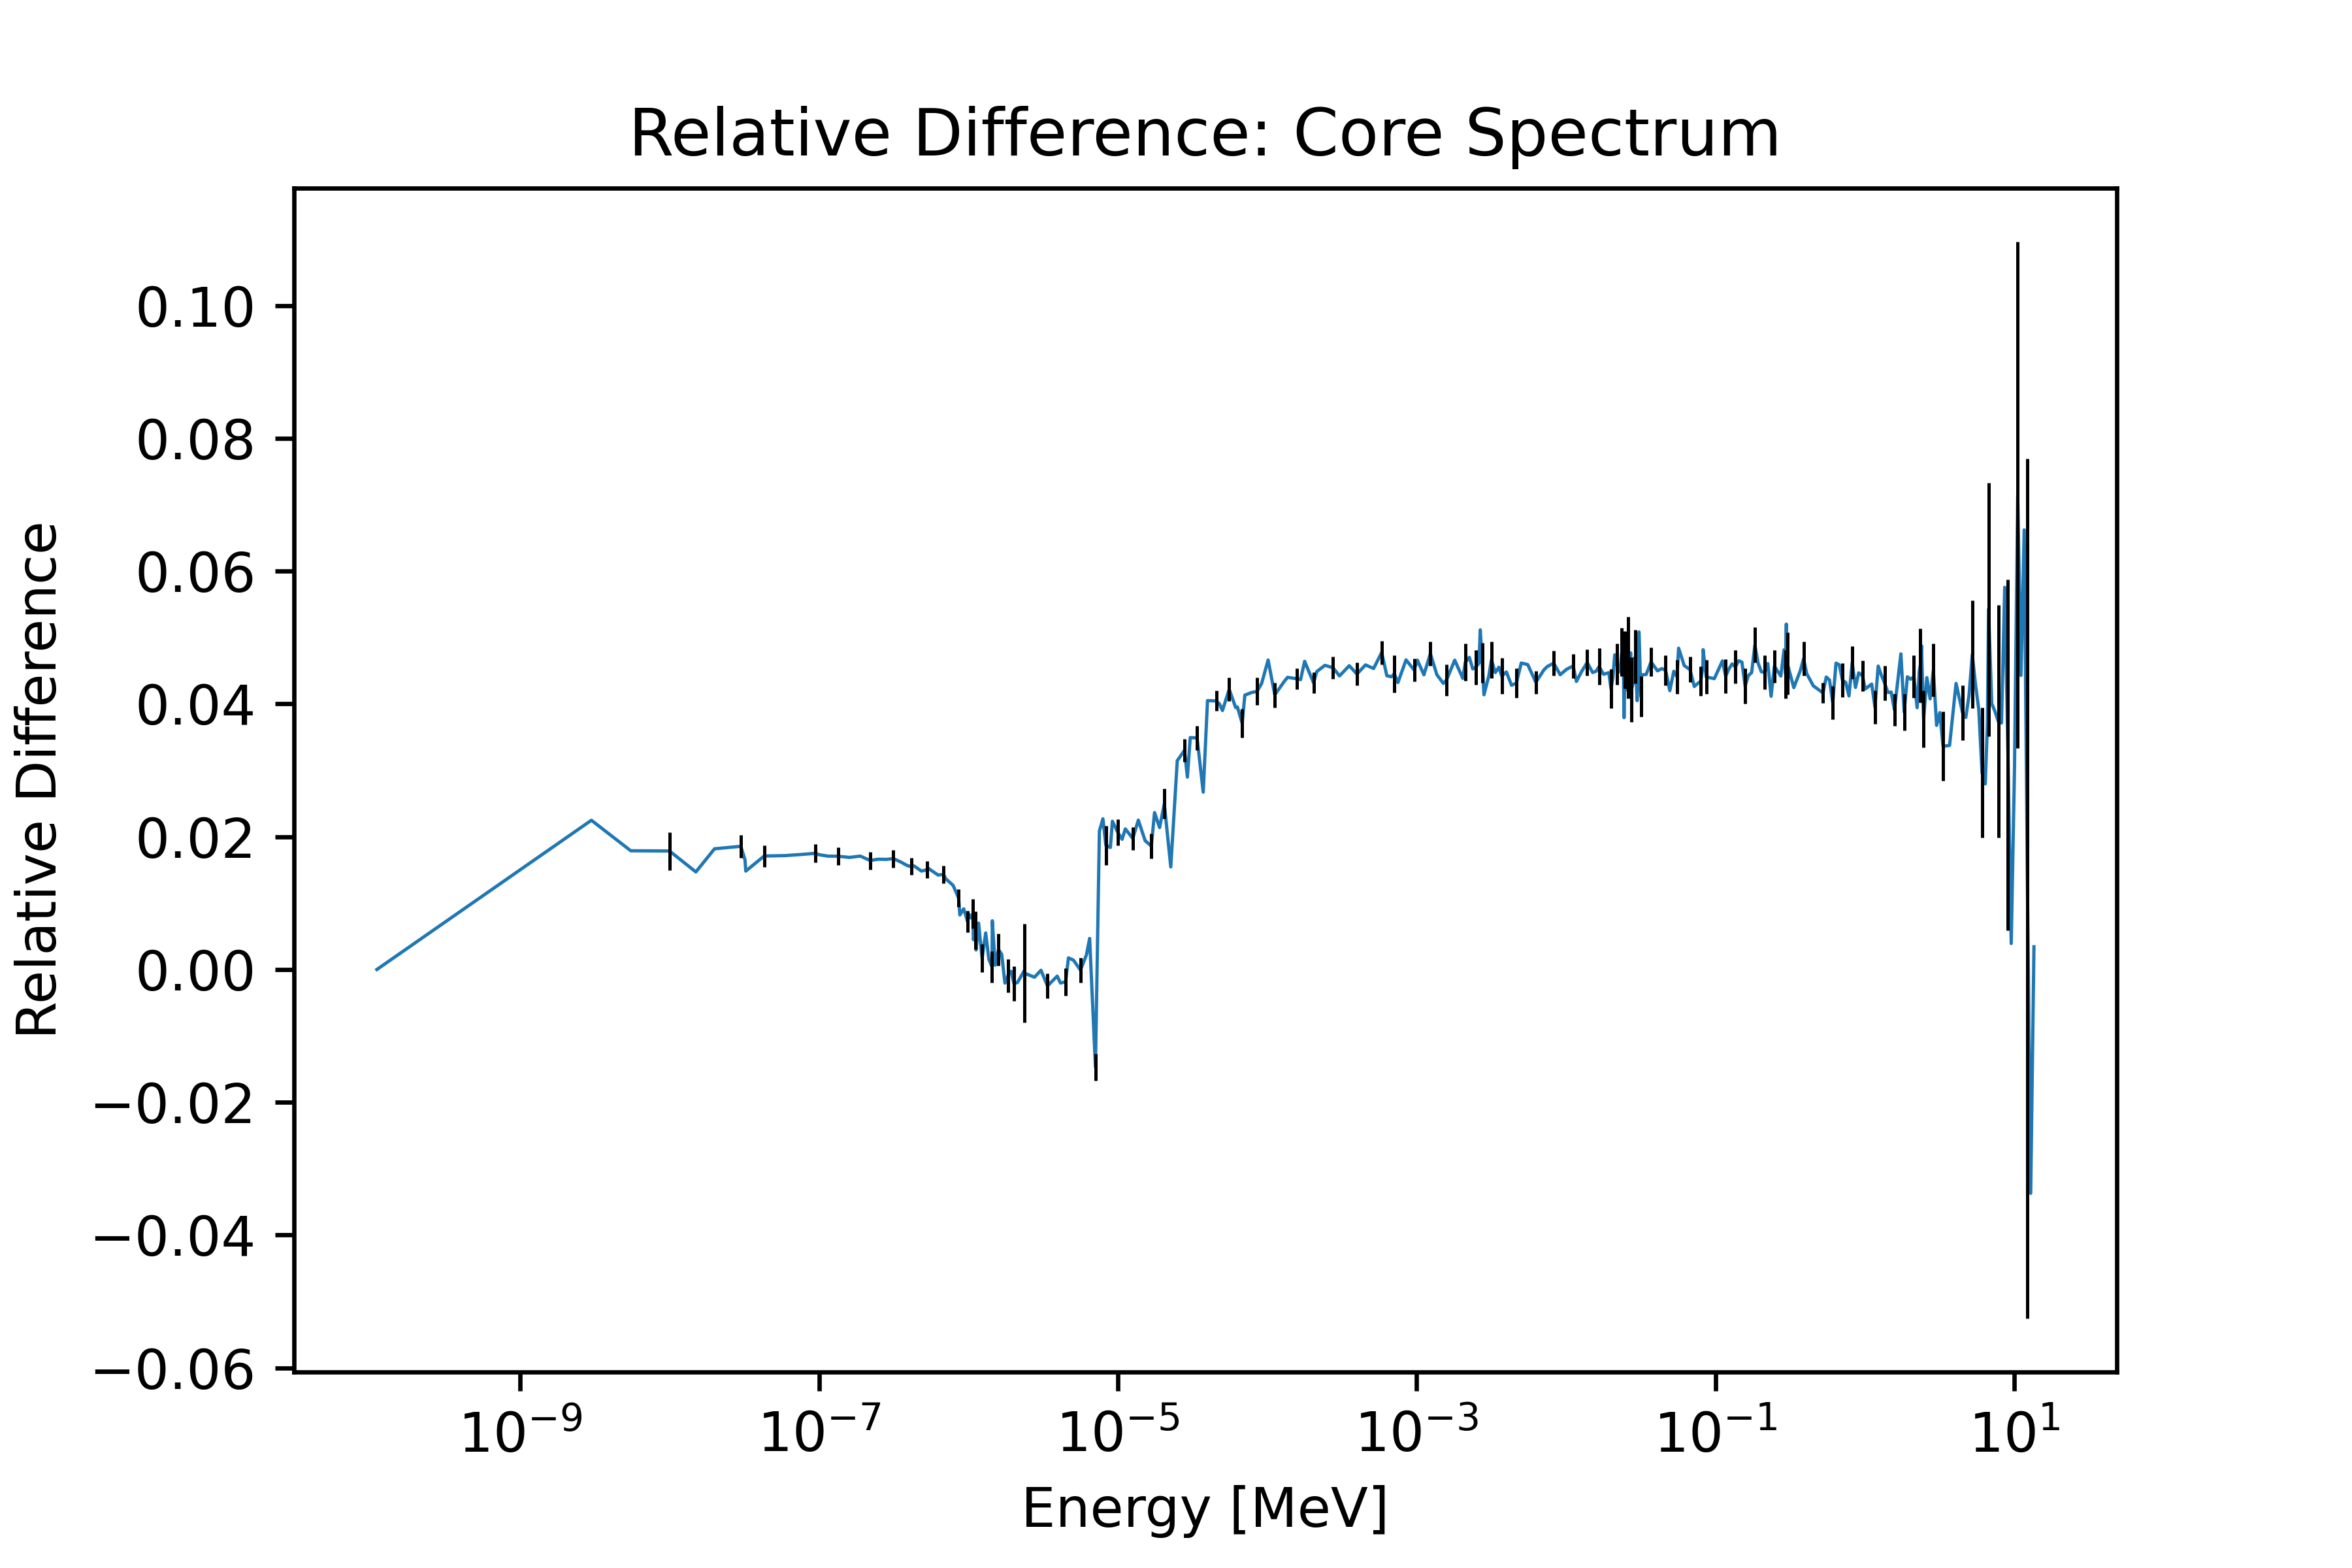
\includegraphics[width=0.95\linewidth]{figures/reldiff_core_spec_er}
  \caption{Core}
  \label{fig:diff-core}
\end{subfigure}%


\begin{subfigure}{0.95\textwidth}
  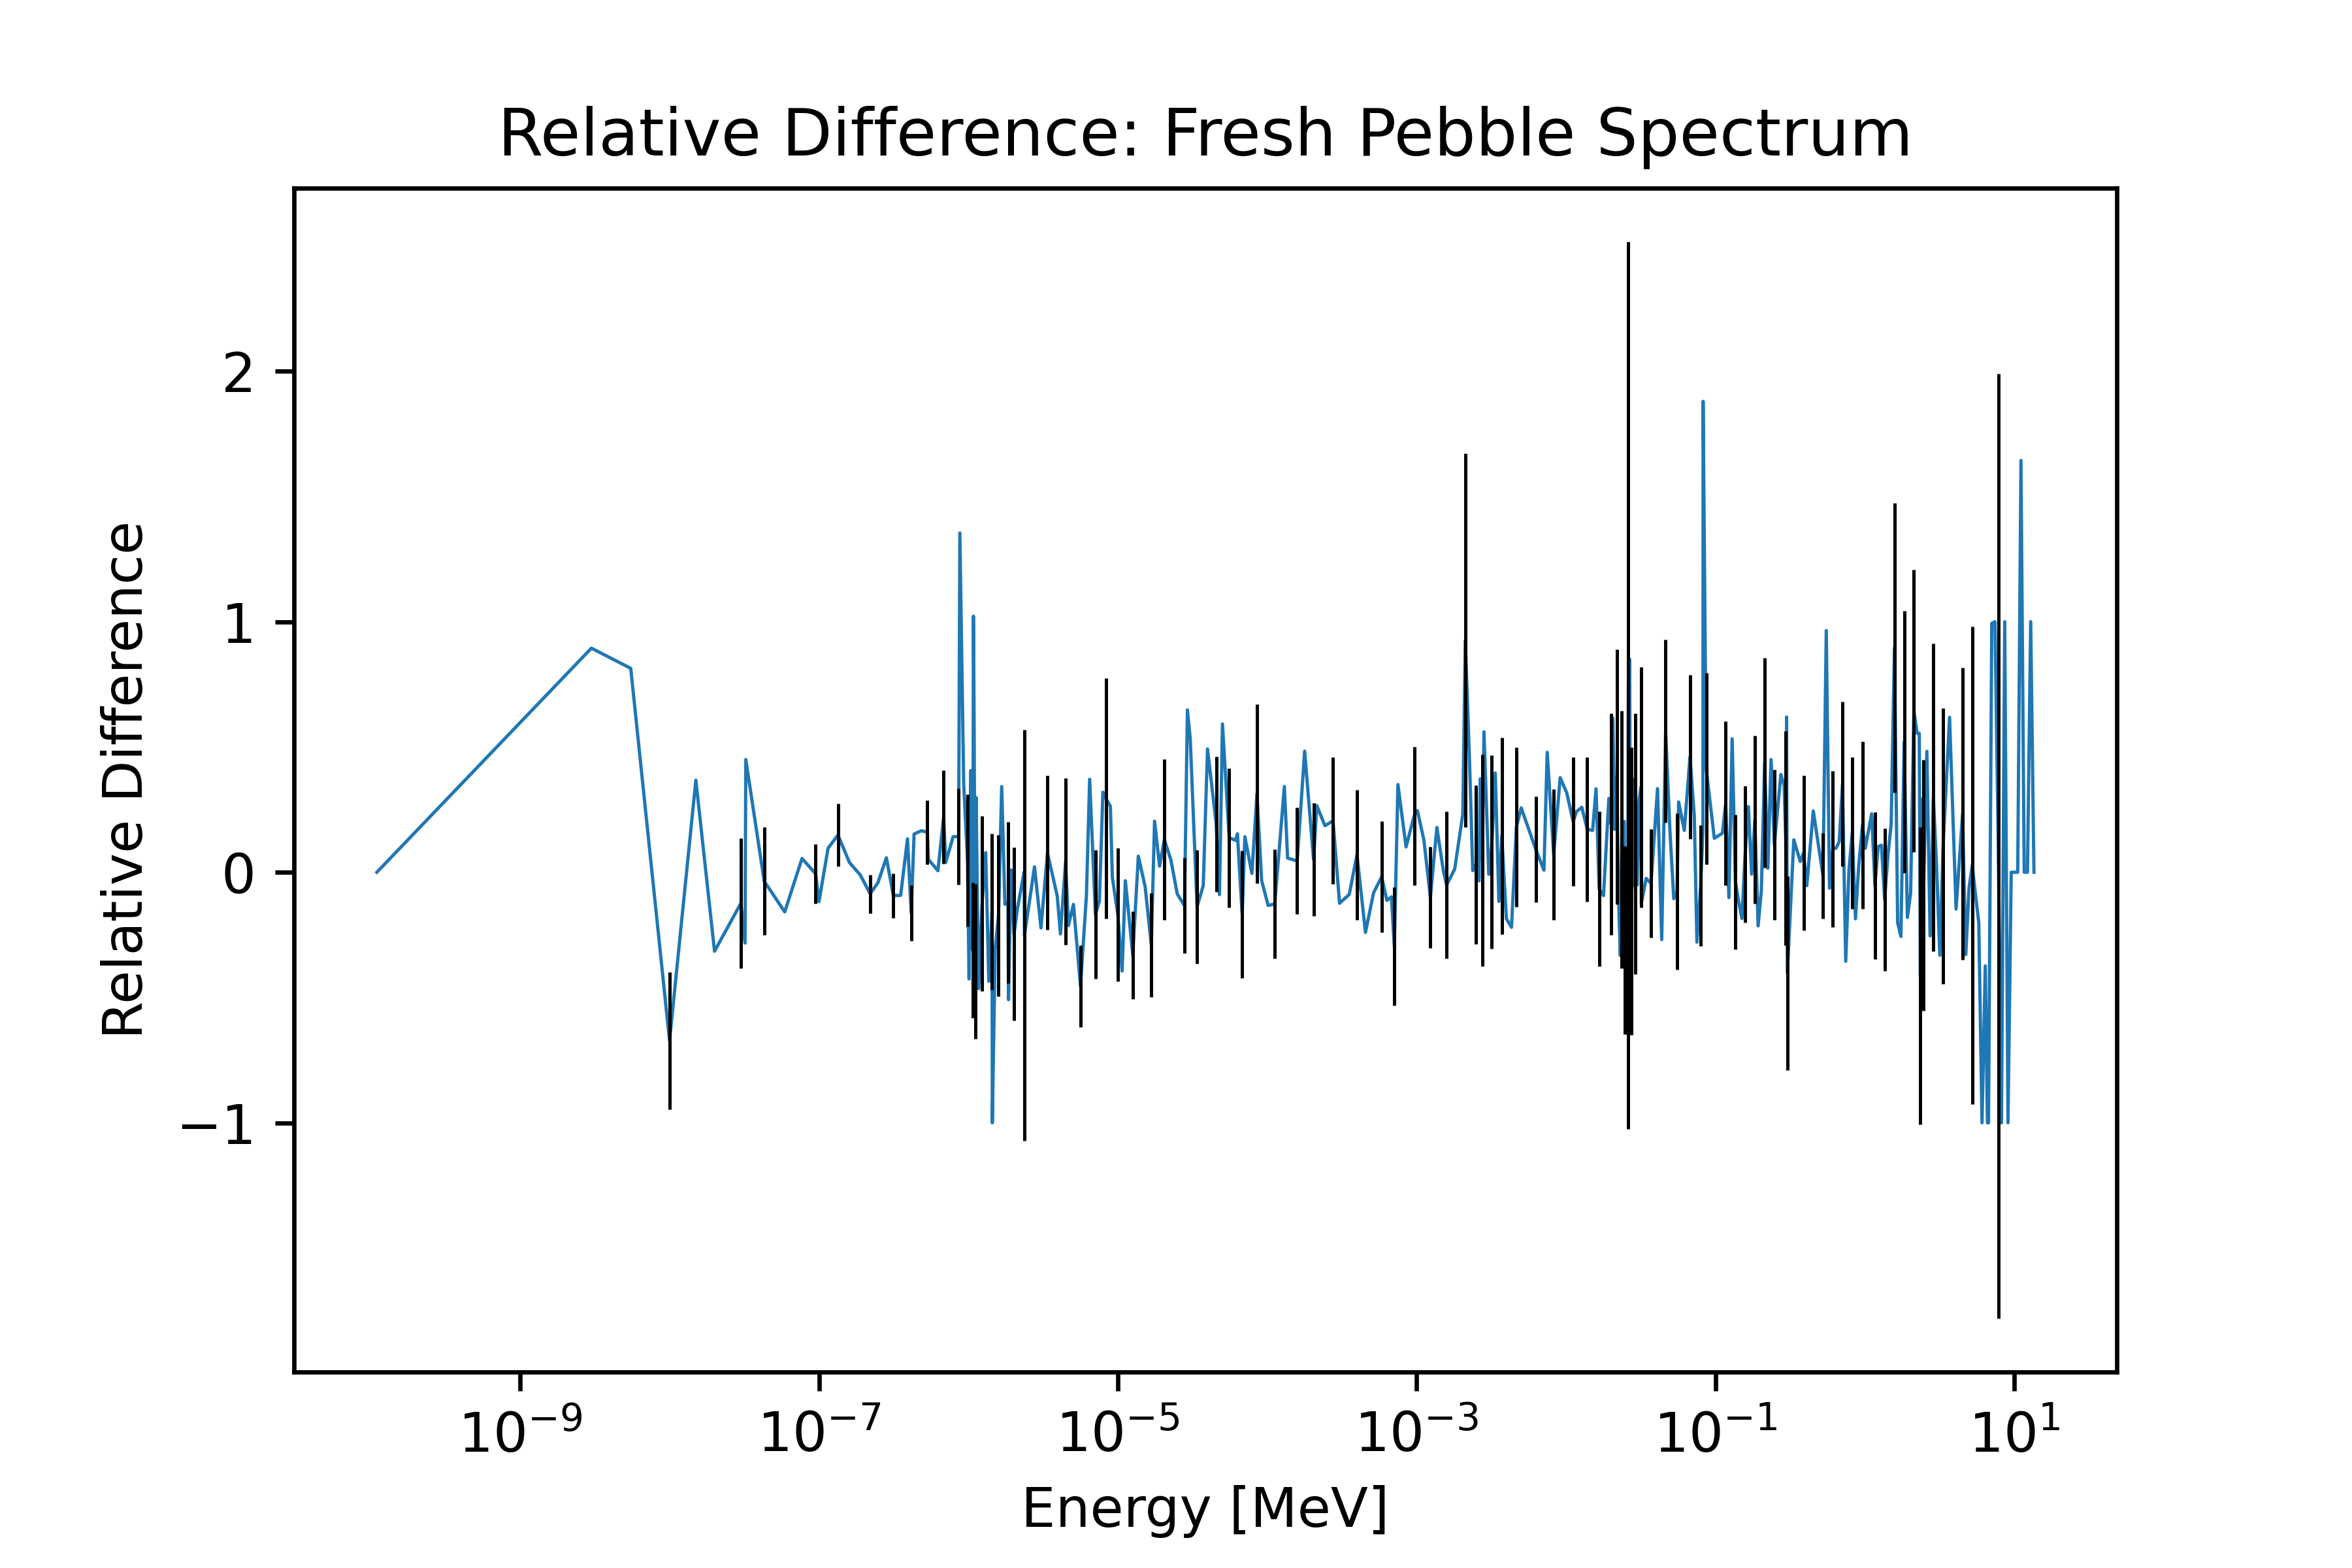
\includegraphics[width=0.95\linewidth]{figures/reldiff_fresh_spec_er}
  \caption{Fresh Pebble}
  \label{fig:diff-fresh}
\end{subfigure}%

\caption{Relative Difference in Lethargy Adjusted Neutron Flux Energy Spectra Between Cores using Homogenized and Heterogenized Pebbles}
\end{figure}

\begin{figure}[H]\ContinuedFloat
\centering

\begin{subfigure}{0.95\textwidth}
  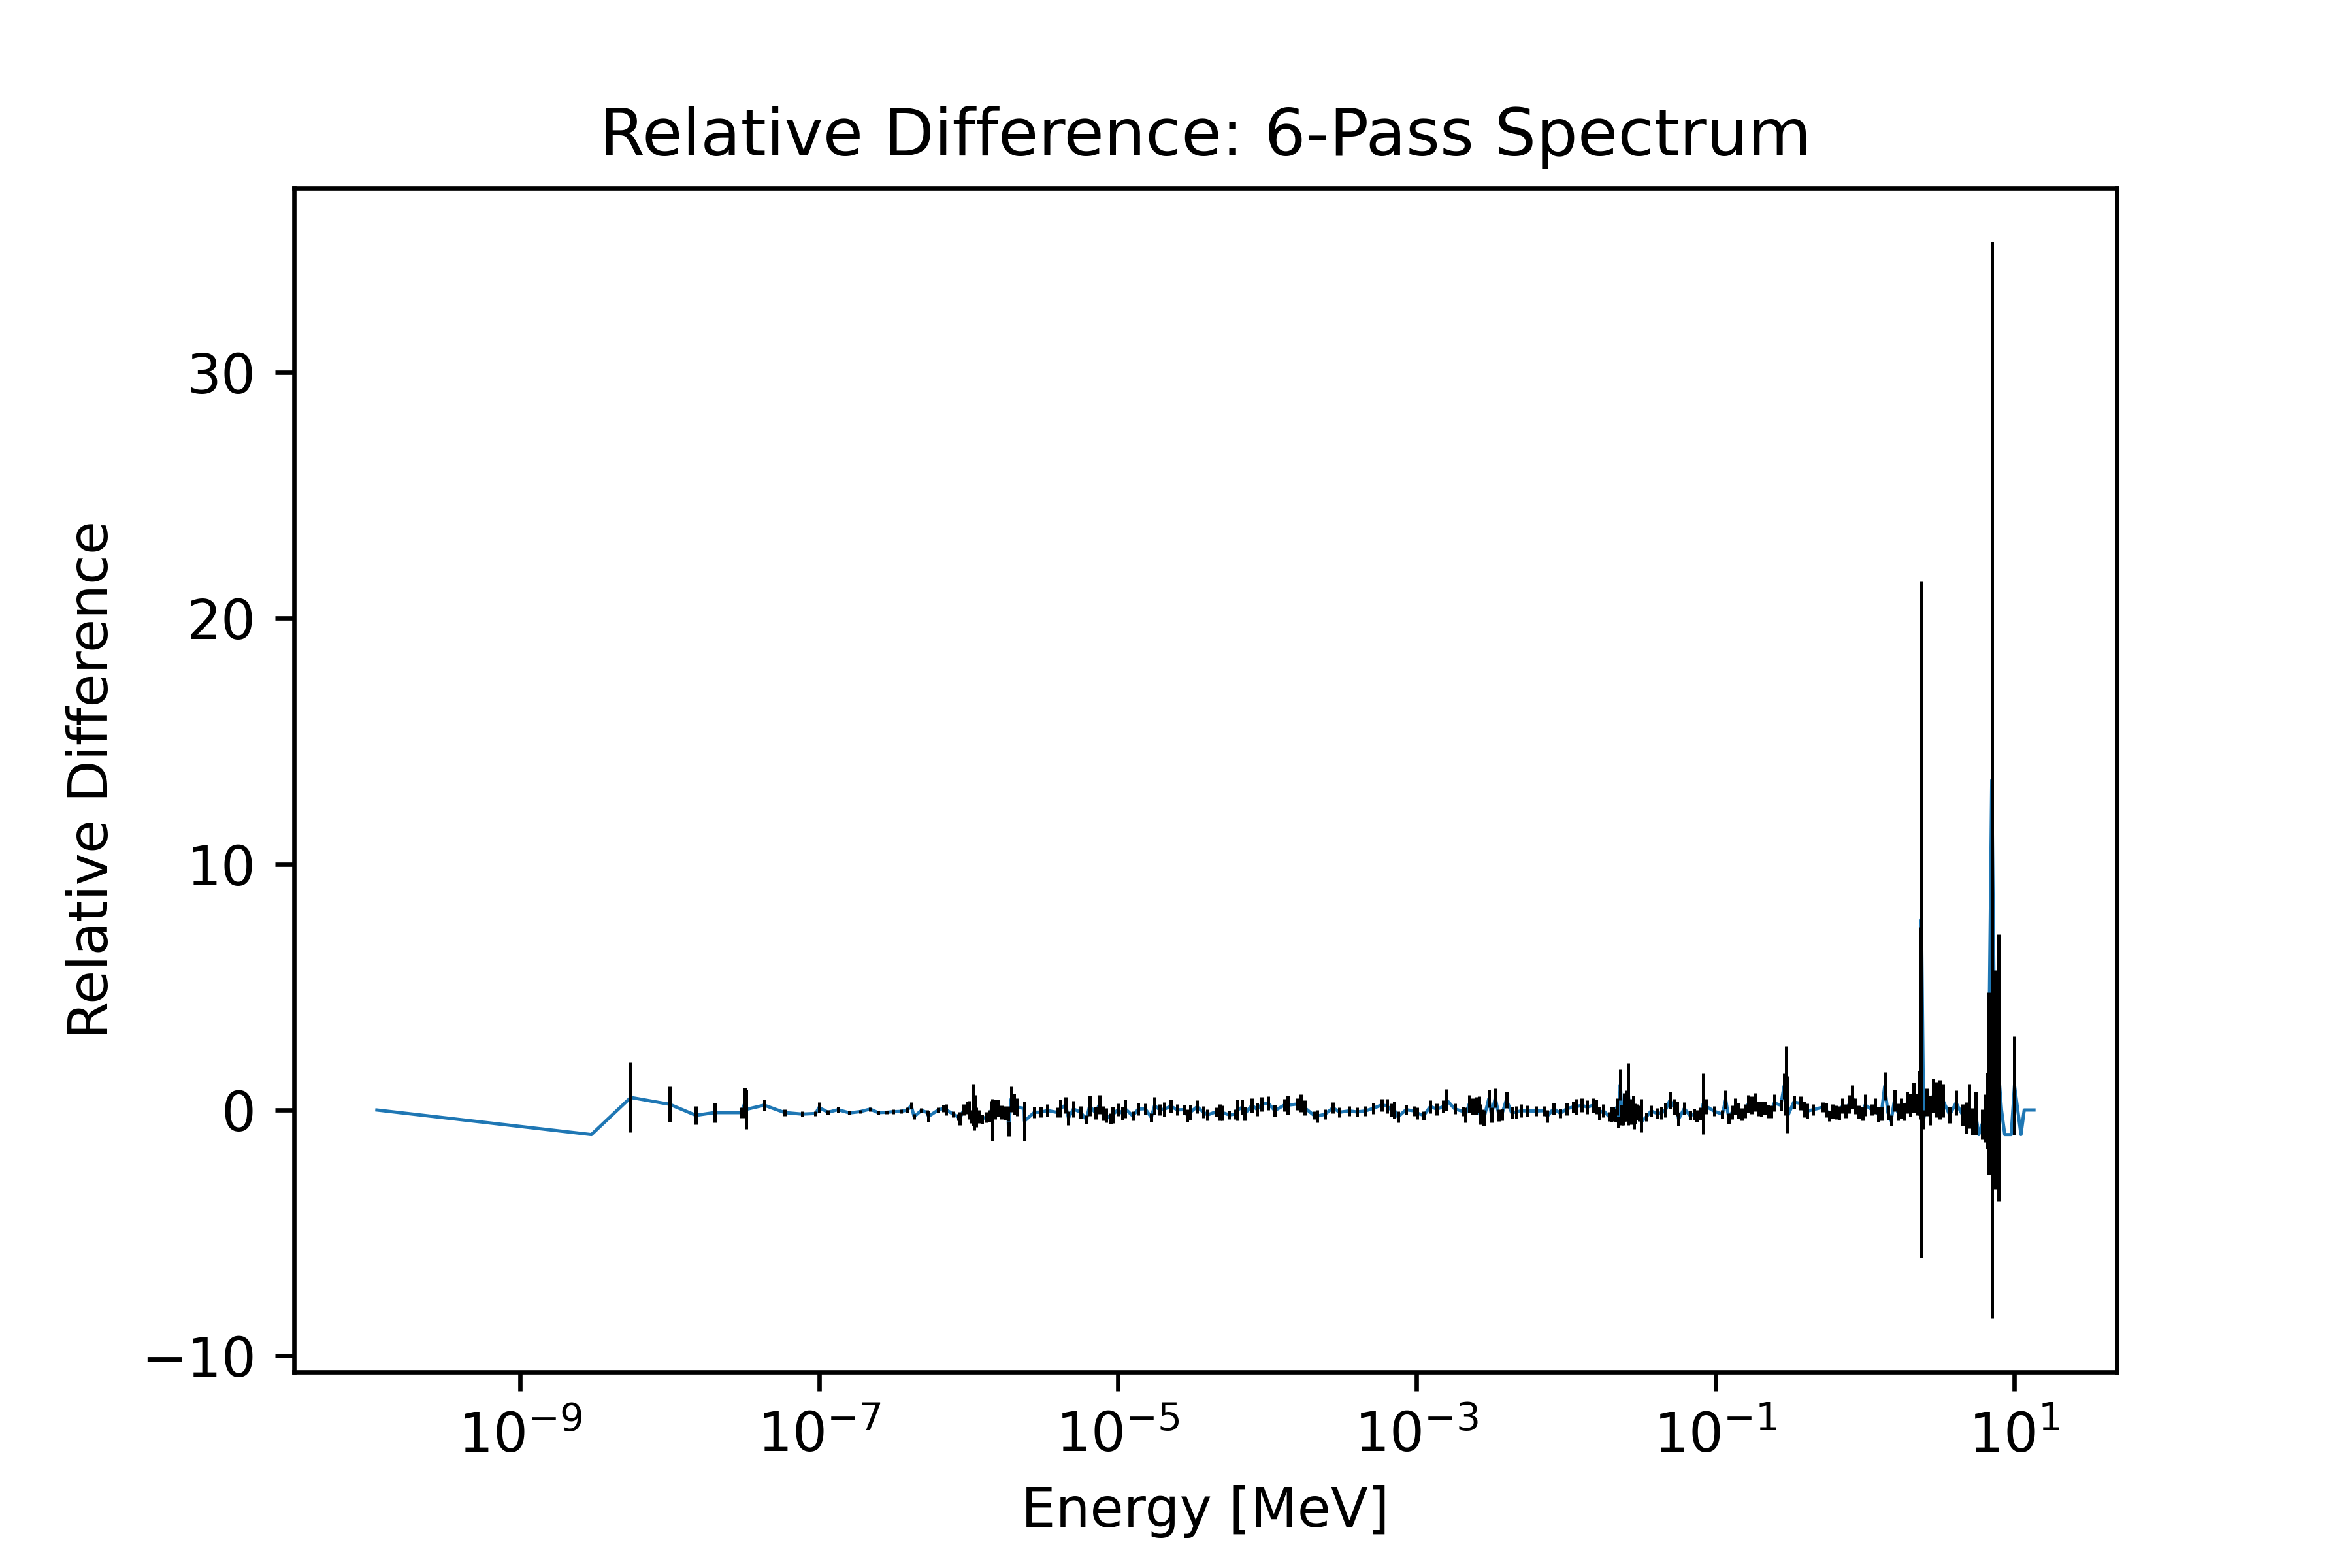
\includegraphics[width=0.95\linewidth]{figures/reldiff_six_spec_er}
  \caption{Six-Pass Pebble}
  \label{fig:diff-six}
\end{subfigure}%


\begin{subfigure}{0.95\textwidth}
  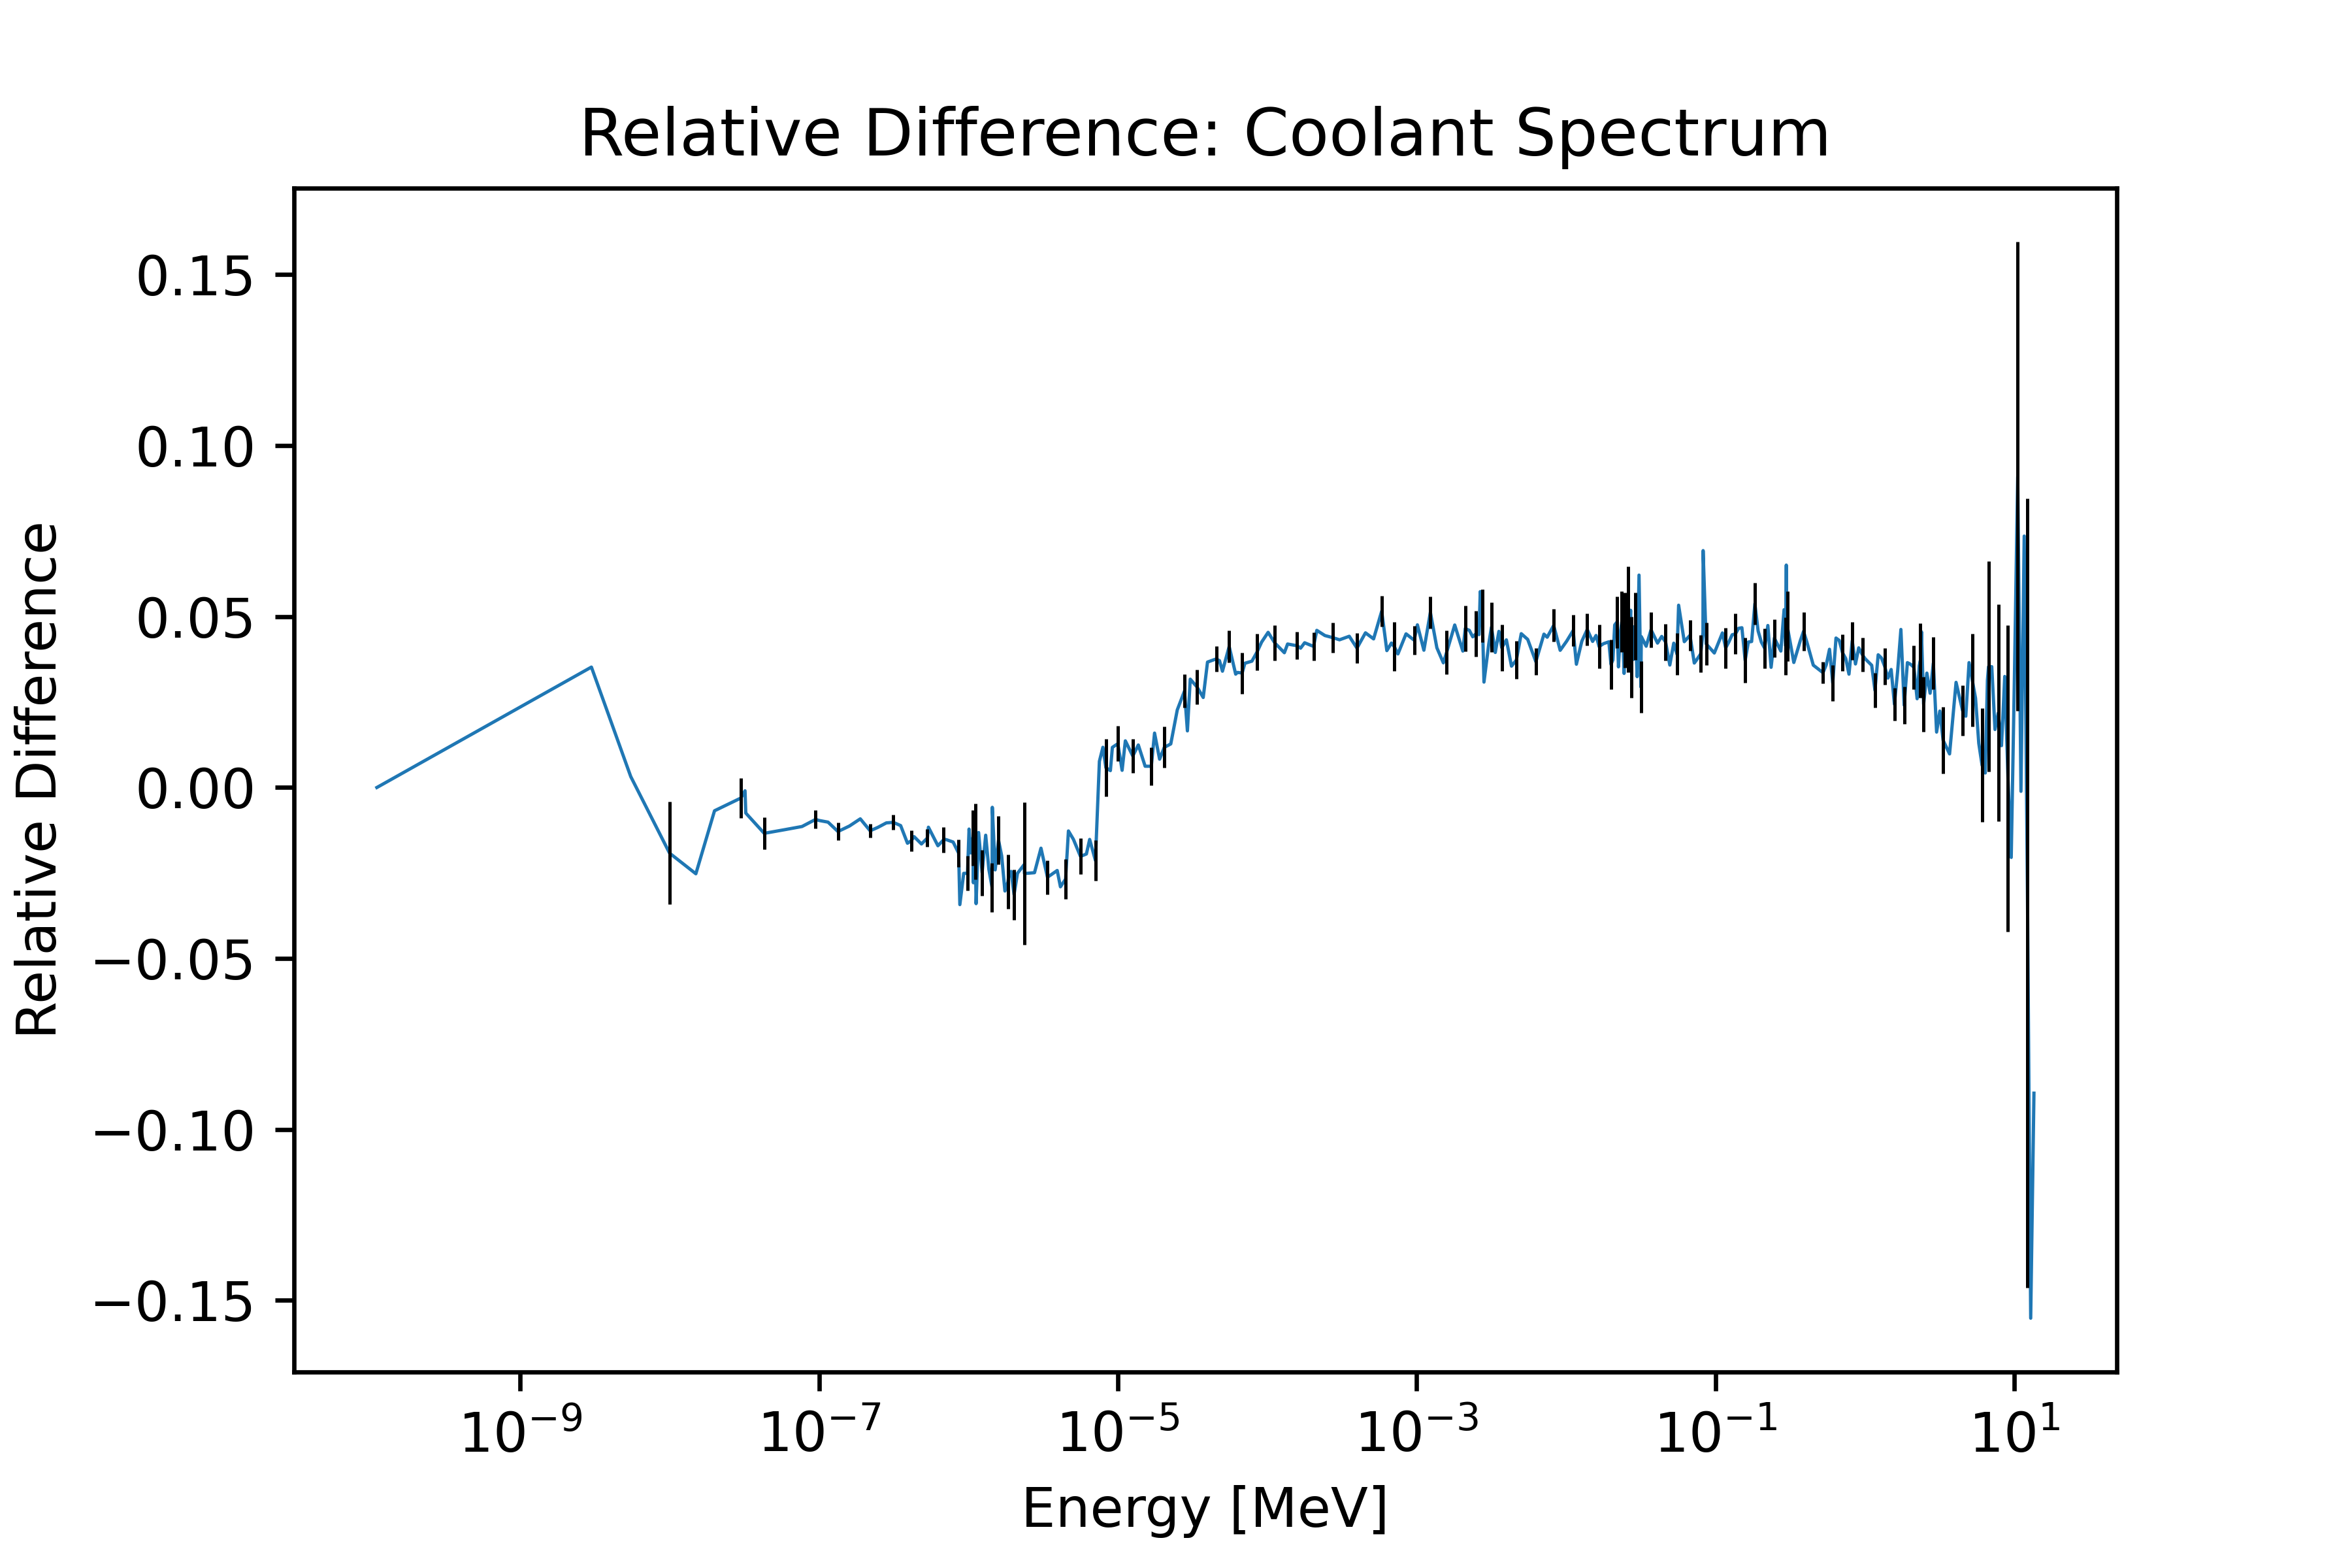
\includegraphics[width=0.95\linewidth]{figures/reldiff_cool_spec_er}
  \caption{Coolant}
  \label{fig:diff-cool}
\end{subfigure}%

\caption[]{(cont.)}
\end{figure}

\begin{figure}[H]\ContinuedFloat
\centering

\begin{subfigure}{0.95\textwidth}
  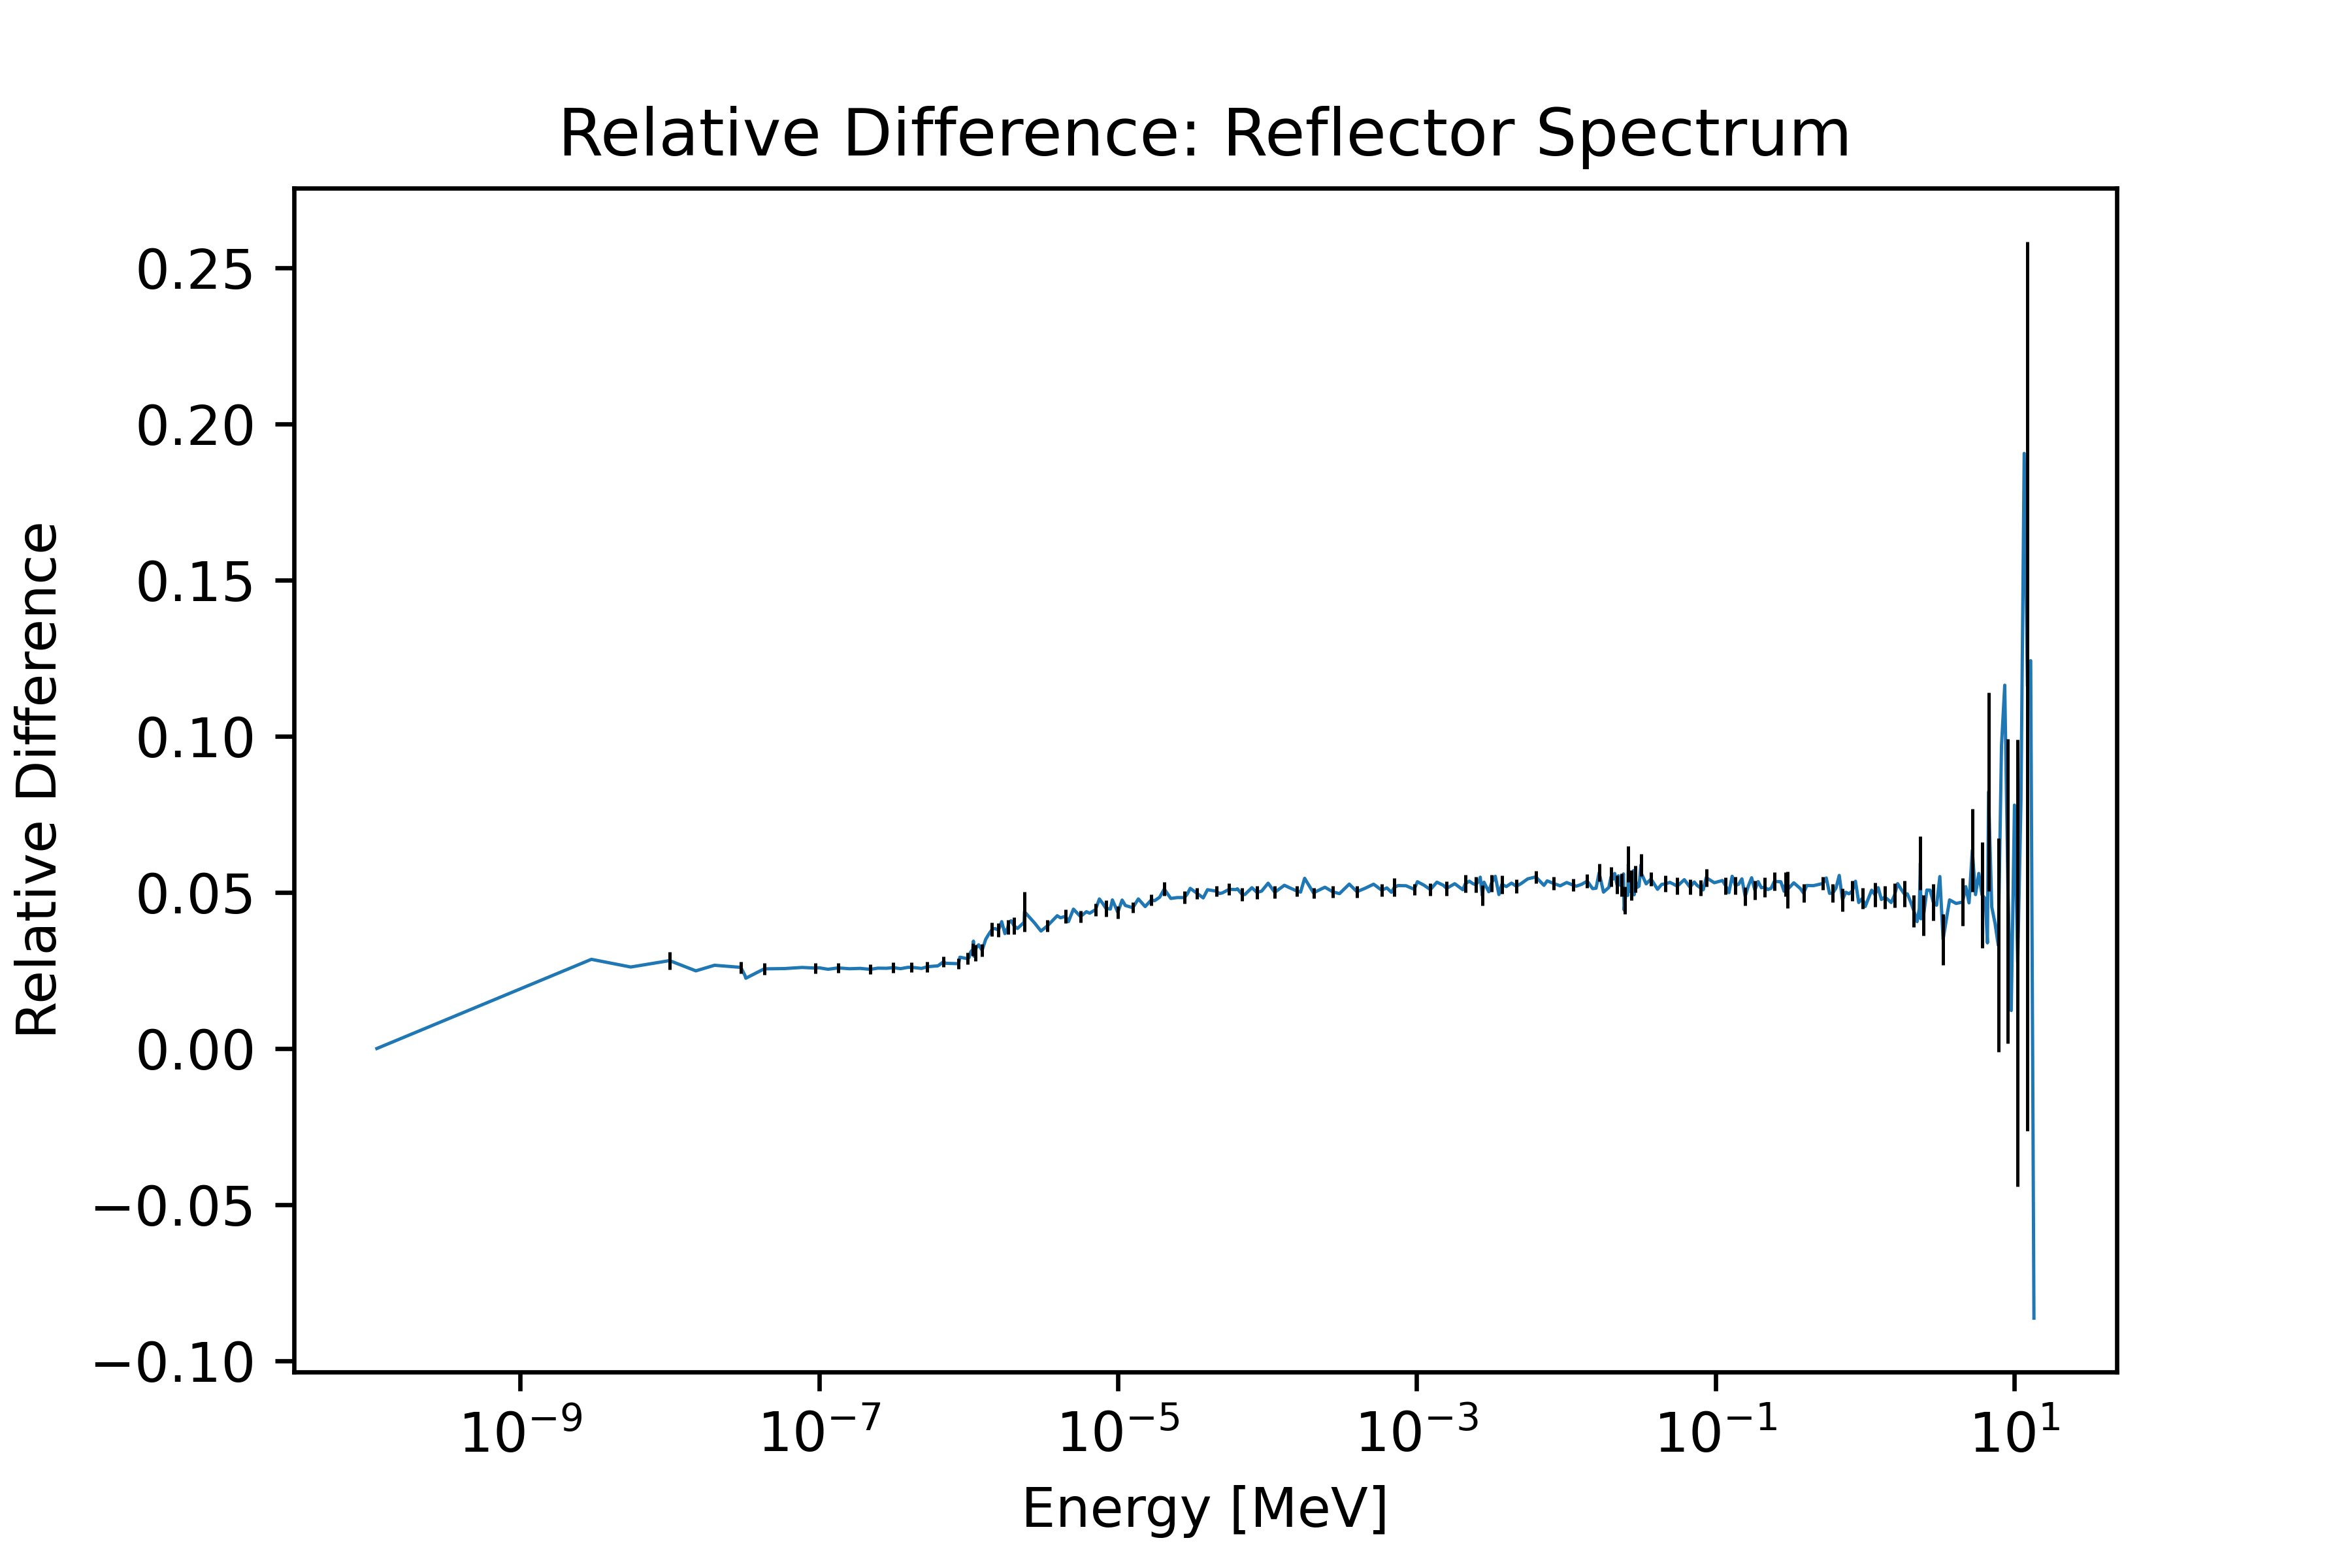
\includegraphics[width=0.95\linewidth]{figures/reldiff_reflec_spec_er}
  \caption{Reflector}
  \label{fig:diff-reflec}
\end{subfigure}%

\caption[]{(cont.)}
\label{fig:diff-spec}
\end{figure}